\chapter{Background}
\label{ch:background}

\blockquote{The focus of this chapter is to explain the concept of lexical flexibility, consider its criticisms, and offer a more robust, functionally-grounded definition instead. I first briefly describe how flexible approaches to lexical categories developed as a response to weaknesses in traditional theories of parts of speech. I then survey the landmark studies and important findings on lexical flexibility, along with criticisms of this research. Following that, I summarize approaches to lexical categories from several functionalist perspectives—cognitive linguistics, typology, and construction grammar. I conclude by offering a revised formulation of lexical flexibility which is more in line with this functional research.}

\section{Introduction: Approaches to lexical flexibility}
\label{sec:2.1}

The field of linguistics as a whole, and the subfield of typology in particular, is undergoing a radical shift in how we understand lexical categories, along primarily two dimensions. The first dimension is our understanding of what lexical categories are a property \emph{of}. Early researchers viewed categories as universal properties of both language and languages \addcite{Haspelmath on g-language vs. p-language; add these terms in parentheses}. I call this the \dfn{universalist} position. After Boas, many researchers then came to view categories as language-specific, with patterned similarities across languages. I call this the \dfn{relativist} approach. Most recently, some researchers view categories as typological patterns rather than properties of any particular language. This is the \dfn{typological} position, and the one I adopt here.

The second dimension of historical change in linguistic theories of categories is in the \emph{nature} of the categories themselves. In the Classical tradition, categories were thought to be categorical and well-defined by a set of necessary and sufficient conditions (in the tradition of Aristotle). After the cognitive turn in the 1980s, many linguists came to view categories as prototypal, with some members of a category being more central, or better exemplars, than others. Cognitive research into the nature of idioms then led to the development of construction grammar, which sees language as consisting of a network of constructions rather than monolithic categories. I adopt a constructional approach to categories in this thesis.

These theoretical paradigm shifts are summarized in \exref{ex:2.1}. At each stage of development, there has not been a wholesale displacement of previous theories \addcite{Kuhn}. There are still many who regard word classes as universal and categorical, and the typological-constructional approach is still nascent.

\begin{exe}
  \ex\label{ex:2.1}
  \begin{xlist}
    \ex universal > language-specific > typological
    \ex categorical > prototypal > constructional
  \end{xlist}
\end{exe}

\secref*{sec:2.2} gives a synopsis of these theoretical positions and shows how research on lexical flexibility developed in recognition of the shortcomings of traditional approaches. \secref*{sec:2.3} summarizes the key concepts and findings that have arisen from the research on lexical flexibility. Such research, however, is not without its own shortcomings. \secref*{sec:2.3} also presents the main criticisms that have been leveled against flexible analyses of word classes. \secref*{sec:2.4} then presents an alternate, functionally-oriented approach—the typological-constructional perspective. The final section of this chapter (\secref{sec:2.5}) then applies this functional perspective to formulate an improved definition of lexical flexibility.

\section{Traditional approaches}
\label{sec:2.2}

This section is a necessarily brief history of approaches to lexical categories up until the cognitive turn of the 1980s. It covers the universalist position that developed in the Classical tradition, the relativist position that developed as a result of Boas' cultural relativism, and the structuralist (or \enquote{distributionalist}) position that developed in the tradition of Saussure. Depending on how one understands and applies these different perspectives, none of them are mutually exclusive. It is especially common for linguists to simultaneously hold that lexical categories must be identified on the basis of language-internal evidence alone (the relativist position) and that lexical categories are universal in some sense or another (the universalist position).

\subsection{Universalist}
\label{sec:2.2.1}

Historically and still presently, many researchers assumed that a small set of lexical categories are basic and universal to all languages \parencites[81]{BolingerSears1981}[2]{Croft1991}[32]{Payne1997}[95]{Stassen2011}. The set typically consists of some variation of the following: Noun, Verb, Adjective, Adverb, Pronoun, Adposition, Conjunction, Numeral, and Interjection \parencite[16538]{Haspelmath2001}. This set has its origins in the \pubtitle{Τέχνη Γραμματική} / \pubtitle{Tékhnē Grammatiké} (\tln{The art of grammar}) of the the \nth{2} century B.C.E. grammarian Dionysius Thrax. The \pubtitle{Tékhnē} synthesizes the work of Dionysius' predecessors, describing eight parts of speech for \idx{Ancient Greek}. These parts of speech were based largely on morphological (especially inflectional) criteria \parencite[17--20]{Rauh2010}. The \pubtitle{Tékhnē} was then translated and its model applied to \idx{Latin} in the \pubtitle{Ars Grammatica} of Remnius Palaemon. The \pubtitle{Ars Grammatica} initiated a tradition wherein the languages of Europe and eventually the world \parentext{e.g. \idx{Mandarin}; \parencite{McDonald2013}} were described using both Dionysius' categories (with occasionally additions / subtractions) as well as his method of identifying those categories on the basis of morphological criteria \parencite[20]{Rauh2010}.

Implicit in the Classical method is the assumption that lexical categories are universal in the sense of being instantiated in all languages. However, as European scholars began to encounter non-Indo-European languages (or even non-Romance languages) in both Europe and abroad, this assumption was challenged, as early as the first grammatical descriptions of Irish in the \nth{7} century. At first, these languages either had Classical grammar imposed upon them or were deemed grammatically deficient \parencite[3]{Suarez1983}. Nonetheless, missionary linguists in the early colonial era were indeed aware of the significant grammatical differences between these languages and Latin, and made their best attempts at describing them \parencite[3--4]{Suarez1983}. It is also important to realize that the project of describing the languages in the Americas and other zones of colonial influence was partially contemporaneous with the publication of the first grammars of the vernacular languages of Europe, as illustrated in \figref{fig:grammars} (the data for which are shown in \tabref{tab:grammars}). Between 1524 and 1572, over 100 catechisms, manuals for confession, collections of sermons, grammars, and vocabularies were written in or about ten languages within the Viceroyalty of New Spain alone (an area smaller than present-day Mexico), mostly by Spanish Franciscan and Jesuit missionaries \parencite[2]{Suarez1983}. The task of converting the indigenous peoples to Christianity via the medium of their own languages was so important to the Spanish crown that the first bishop of Mexico, Francisco de Zumárraga, brought a printing press to Mexico in 1534 (just 15 years after the arrival of the first Spaniards in Mexico in 1519). The first book printed in Mexico was a Spanish-Nahuatl catechism by Alonso de Molina \parencite[2]{Suarez1983}. Scholars were wrestling with the lexical categories of non-Indo-European languages at a very early stage.

\begin{figure}
  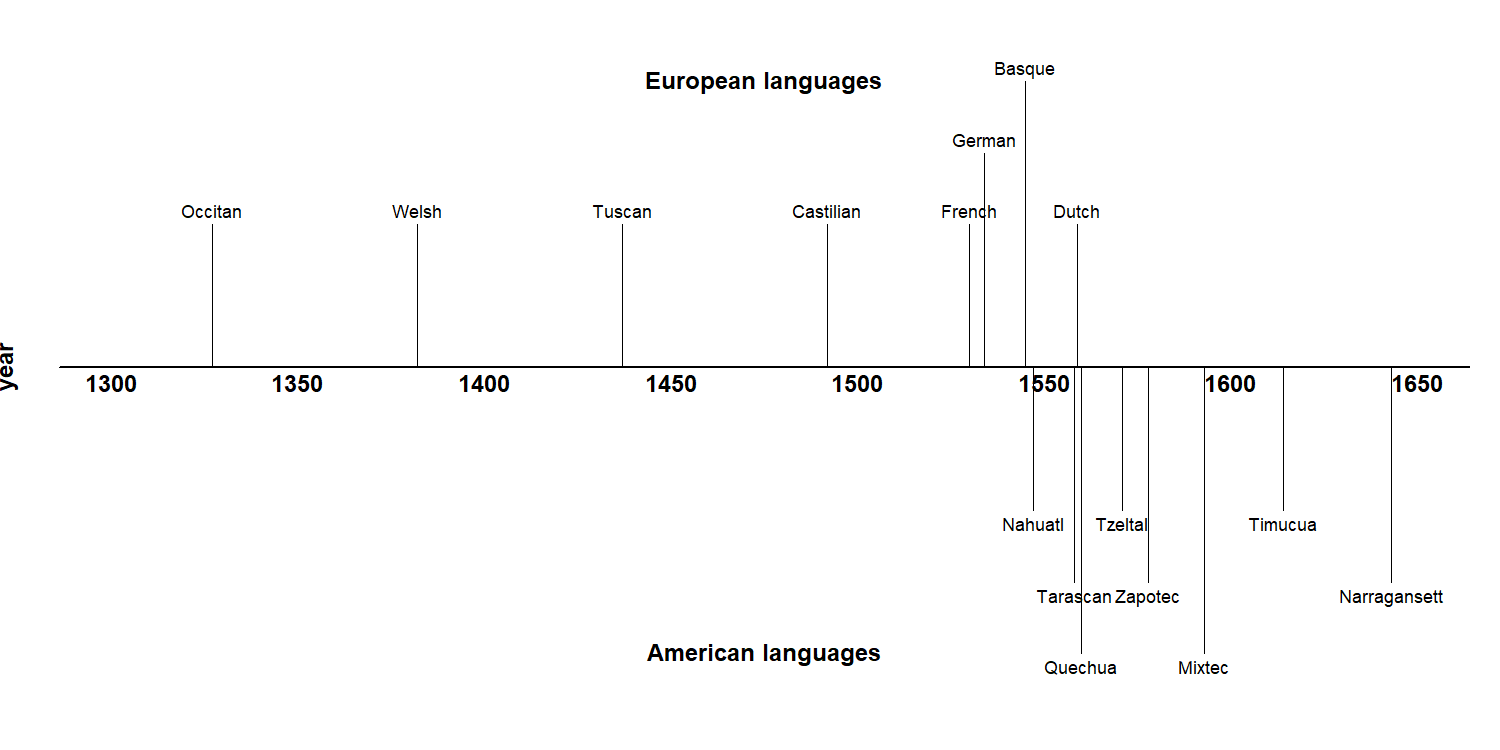
\includegraphics[width=\linewidth]{grammars.png}
  \caption{Approximate date of some of the first grammatical descriptions of European vs. American languages}
  \label{fig:grammars}
\end{figure}

\singlespacing
\setlength\LTleft{0pt}
\setlength\LTright{0pt}
\renewcommand{\arraystretch}{1.5}

\begin{longtable}{ l l l l }
  \caption{Some first grammatical descriptions of European vs. American languages}
  \label{tab:grammars}\\
  \toprule
    Language     & Year       & Title                                                                                                                                                                                         & Author\\
  \midrule
  \endhead
    Irish        & 600s       & \parbox[t]{2.5in}{\pubtitle{Auraicept na n-Éces}\\\tln{The scholars' primer}}                                                                                                                 & Longarad\\
    Occitan      & 1327       & \parbox[t]{2.5in}{\pubtitle{Leys d'amors}\\\tln{Laws of love}}                                                                                                                                & Guilhèm Molinièr\\
    Welsh        & 1382--1410 & \parbox[t]{2.5in}{\pubtitle{Llyfr Coch Hergest}\\\tln{Red book of Hergest}}                                                                                                                   & unknown\\
    Tuscan       & 1437--1441 & \parbox[t]{2.5in}{\pubtitle{Grammatica della lingua toscana}\\\tln{Grammar of the Tuscan language}}                                                                                           & Leon Battista Alberti\\
    Castilian    & 1492       & \parbox[t]{2.5in}{\pubtitle{Gramática de la lengua castellana}\\\tln{Grammar of the Castilian language}}                                                                                      & Antonio de Nebrija\\
    French       & 1530       & \parbox[t]{2.5in}{\pubtitle{L'Éclaircissement de la langue francoyse}\\\tln{Explication of the French language}}                                                                              & John Palsgrave\\
    German       & 1534       & \parbox[t]{2.5in}{\pubtitle{Ein Teutsche Grammatica}\\\tln{A German grammar}}                                                                                                                 & Valentin Ickelsamer\\
    Basque       & 1545       & \parbox[t]{2.5in}{\pubtitle{Linguæ Vasconum Primitiæ}\\\tln{First fruits of the Basque language}}                                                                                             & Bernard Etxepare\\
    Nahuatl      & 1547       & \parbox[t]{2.5in}{\pubtitle{Arte para aprender la lengua mexicana}\\\tln{Grammar for learning the Mexican language}}                                                                          & Bernard Etxepare\\
    Tarascan     & 1558       & \parbox[t]{2.5in}{\pubtitle{Arte de la lengua tarasca de Michoacán}\\\tln{Grammar of the Tarascan language of Michoacán}}                                                                     & Maturino Gilberti\\
    Dutch        & 1559       & \parbox[t]{2.5in}{\pubtitle{Den schat der Duytsscher Talen}\\\tln{The treasure of the Dutch language}}                                                                                        & John III van de Werve\\
    Quechua      & 1560       & \parbox[t]{2.5in}{\pubtitle{Grammatica o arte de la lengua general de los Indios de los Reynos del Peru}\\\tln{Grammar or Art of the General Language of the Indians of the Royalty of Peru}} & Domingo de Santo Tomás\\
    Tzeltal Maya & 1571       & \parbox[t]{2.5in}{\pubtitle{Ars Tzeldaica}\\\tln{Tzeltal Grammar}}                                                                                                                            & Fray Domingo de Hara\\
    Zapotec      & 1578       & \parbox[t]{2.5in}{\pubtitle{Arte en lengua Zapoteca}\\\tln{Grammar in the Zapotec language}}                                                                                                  & Juan de Córdova\\
    English      & 1586       & \parbox[t]{2.5in}{\pubtitle{Pamphlet for Grammar}}                                                                                                                                            & William Bullokar\\
    Mixtec       & 1593       & \parbox[t]{2.5in}{\pubtitle{Arte de lengua Mixteca}\\\tln{Grammar of the Mixtec language}}                                                                                                    & Antonio de los Reyes\\
    Timucua      & 1614       & \parbox[t]{2.5in}{\pubtitle{Gramatica de la lengua Timuquana de Florida}\\\tln{Grammar of the Timucua language of Florida}}                                                                   & Francisco Pareja\\
    Narragansett & 1643       & \parbox[t]{2.5in}{\pubtitle{A key into the language of America}}                                                                                                                              & Roger Williams\\
  \bottomrule
\end{longtable}

\renewcommand{\arraystretch}{1}
\doublespacing

These categories were thought to be basic in the sense of either a) being universally instantiated in all languages, or b) being universal categories available to all languages, but only instantiated in some (Hieber 2013: {{p. ??}})

\subsection{Relativist}
\label{sec:2.2.2}

\subsection{Structuralist}
\label{sec:2.2.3}

\section{Flexible approaches}
\label{sec:2.3}

\section{Functional approaches}
\label{sec:2.4}

\section{Lexical flexibility: A functional definition}
\label{sec:2.5}
